\chapter{Methodology}\label{cha:methodology}

    In the spirit of reproducibility, this chapter describes the tools and procedures used in the development of this project. Starting with the hardware, the requirements for this project were minimal. An Intel\textsuperscript{\textregistered} Core\texttrademark\ i7-1065G7 CPU 1.30 GHz processor with a memory capacity of 15.2 GiB of RAM was used. The operating system consisted of Ubuntu 22.04. A system with substandard specifications can also be adequate for development.

\section{Development Environment}

    For the sake of simplicity and to isolate the development environment from global dependencies, a \textsf{conda} environment was created. This \textsf{conda} environment was used to build the \ac{ROS} packages required. The essential packages installed in the development environment are shown in Table~\ref{tab:envdeps}. For quick installation, an environment yaml file is provided at TODO

    \begin{table}[htbp]
        \color{textColor}
        \centering	
        \caption{Development environment dependencies}

        \begin{tabular}{lc}
            \toprule
            \textbf{Package} & \textbf{Version} \\
            \midrule
            \textsf{python} & $3.10$ \\

            \textsf{setuptools}\tablefootnote{Version $58.2.0$ of \textsf{setuptools} is the highest version that supports \textsf{setup.py} installs which many of the core ROS packages depend upon.} & $58.2.0$ \\

            \textsf{numpy} & $1.24$ \\ 

            \textsf{lark}\tablefootnote{The \textsf{lark} package is required for \textsf{builtin}\texttt{\_}\textsf{interfaces}} & $1.1$ \\

            \textsf{rosdep} & $0.22$ \\

            \textsf{cmake} & $3.25$ \\

            \textsf{colcon-core} & $0.12$ \\

            \textsf{colcon-ros} & $0.3$ \\

            \textsf{colcon-package-selection} & $0.2$ \\

            \textsf{colcon-devtools} & $0.2$ \\

            \textsf{nodejs} & $18.12$ \\

            \bottomrule
                
        \end{tabular}\label{tab:envdeps}
    \end{table}


\section{Compilation Tools}

    Given that the \textsf{colcon} package is already well adapted to build ROS packages, \textsf{colcon} was widely used throughout this project with a few customizations. 
    In order to cross-compile the \ac{ROS} C++ and C packages to WebAssembly, the \ac{emsdk} version $3.1$ was installed. The Emscripten toolchain was then provided to \textsf{colcon} as a \textsf{cmake} argument (See Appendix~\ref{sec:apxblasm} Line $109$).


\section{Package Building Process}

    Before any packages could be built, all of the ROS 2 core packages were cloned in a local workspace. To prevent compilation issues, packages related to the default middleware implementations were excluded by adding a \textsf{COLCON}\texttt{\_}\textsf{IGNORE} file in their respective root directories; these include \textsf{iceoryx}, \textsf{cyclonedds}, \textsf{fastrtps}, and \textsf{connextdds}. A secondary purpose for excluding these packages is to ensure that the custom middleware implementation is the only implementation available at runtime. This custom middleware implementation must also be included in the current workspace before proceeding. 

    Additionally, a ``blasm'' script was created to aid in the building of packages given that the number of arguments quickly became exceedingly lengthy for manual input. The entire script is included in Appendix~\ref{sec:apxblasm} for reference. With this script, it is possible to build any package and its dependencies, or to build a package individually. Care must be taken to ensure that the environment variables for the tools such as \textsf{EMSDK}\texttt{\_}\textsf{DIR} are set accordingly. The list of options for this script are shown in Figure~\ref{fig:blasm}.

    \begin{figure}[htbp]
        \centering
        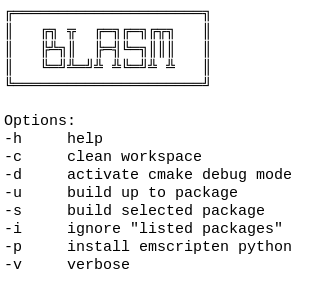
\includegraphics[width=0.4\textwidth]{04_blasm.png}
        \caption{Blasm script options.}
        \label{fig:blasm}
    \end{figure}


    If the package compiles without errors, any executables in the package will be converted to \textit{.wasm} and \textit{.js} files to be run on the browser.


\section{Debugging Tools}

    When working with new ROS packages, there are two main sources of errors: errors during compilation and errors at runtime. To tackle compilation errors, the first step is to obtain a full description of the error. The ``blasm'' script has the option to dynamically activate verbose (\textsf{-v}) mode as needed.

    Secondly, for debugging errors at runtime, one of the most effective tools is the use of logs. Core \ac{ROS} packages such as \textsf{rcutils} and \textsf{rcpputils} already include logging functionalities. Adapting these \ac{ROS} logs into any newly created packages allows for efficient and quick debugging. Alternatively, customized logging functions could be implemented for an in-depth analysis at the expense of increasing the complexity of the package in question.

\section{Post Processing}

    Once the executables have been successfully compiled, the generated JavaScript files are augmented with additional functions to enable communication between the main thread and the ROS packages. The added functions are described in Appendix~\ref{sec:apxmodule}. (TODO: OR provide link to file on GitHub)

\section{Testing Environment}

    Lastly, there are two phases of testing. The first phase consists of testing the packages directly from the terminal. For the early stages such as during the replacement of the middleware implementation, cross-compilation is not yet required; thus, it is possible to locally test the middleware packages by comparing their behavior with the default middleware implementations. This can be achieved in a separate \textsf{conda} environment with \ac{ROS} 2 packages preinstalled by creating and installing an overlay which only includes the customized middleware implementation.

    And the second phase involves testing the packages on a web browser. For this project, only Firefox and Chrome were subject to testing due to their popularity. The tools developed in this project may be suitable for other browsers, however, their full functionality is not guaranteed.
